\documentclass{sig-alternate-05-2015}
\usepackage{subcaption}
\begin{document}

\author{Alun Meredith\vspace{-2ex}% Toggle commenting out the command
}
\date{March 17, 2016 \vspace{-4ex}}
\title{Text Mining \vspace{-2ex}% to see the effect
}
\maketitle
\small


\maketitle

\section{Introduction}
The corpus analysed is a collection of 24 books about antiquity, written in the 18-19th Century. Many are translations of older texts and often volumes of a larger book. The data is html documents of OCR scans from the Google Books Library Project, separated into each page.

Manually extracting some metadata about each book (title, author, translator, year written, year translated) we can see some themes worth investigating: If it is written about/by a Roman or not, written in/about antiquity, volumes within a series, written by the same author, effect of different translators.

\section{Pre-Processing}
To extract the text from each html page, xml2\cite{xml2} was used. Using html tags to isolate the second paragraph (class = 'ocr\_par'), which contained the body of text without the title. The 'ocr\_cinfo' class contained each word separately to avoid an error where words across newlines were merged with a naive approach. Pages were concatenated to produce books.

Using the 'tm' package\cite{tm} a raw corpus was built from these vectors. After casefolding; whitespace, non-alphabetic characters and stopwords were removed. Stopwords removed were tm's "english", numbers and common artefacts of the OCR. A regular expression was used to remove Roman numerals and words were stemmed.

To produce a term-document matrix (tdm) of 1-3 ngrams: sparse terms where removed, a restriction that terms must occur at least 5 times was introduced, to reduce the effect of random occurances of words and reduce size of the tdm. Term frequency - inverse document frequency was used to weight terms based on their background frequency, although our corpus is a biased judge of background frequency considering large portions written by same few individuals.\footnote{Different levels of sparsity used for some purposes, value of 0.95 used if not stated, i.e. term must be present in at least 2 documents.} It is important that the document term matrix is normalised, taking into account the different sizes of the documents. Finally a cosine dissimilarity matrix was computed. Many of the algorithms act directly upon this matrix rather than the tdm. 

\section{Entropy}
The Shannon empirical entropy \cite{shannon2001mathematical}\cite{entropy} was computed on each book using the "entropy" package before the stopwords had been removed using the entropy package conducted on corpus without stop word removal. 

\begin{figure}
\centering
\includegraphics[width=0.7\linewidth]{entropy.png}
\caption{Shannon Entropy of each document, coloured by book each volume belongs to. Full names on github}
\vskip -6pt
\label{fig:entropy}
\end{figure} 

Within the 5 terms with the highest entropy are the dictionary/encyclopedia style books which are expected to have the highest information density. In addition volumes of the same book are generally ranked close together with the exception of Josephus IV and Tacitus History IV, the later of which is quite a remarkable outlier. Cases where the translator changes for volumes of the same book doesn't have a noticeable impact (E.g. Decline \& Fall 4 vs. 1,3,5). This suggests there isn't a strong component of things being translated in totally different ways. 


\section{Clustering} 
Agglomorative hierarchical clustering was evaluated against the cosine dissimilarity matrix using the cluster package \cite{kaufmanpj}\cite{cluster}(fig. \ref{fig:heir}). "Ward" method was used although other methods were tested with the same results (except single linkage). 

Unlike the entropy measure which grouped volumes of a book together well, hierarchical clustering with TF-IDF is grouping on topic rather than language style. There are 3 main clusters, looking at their highly weighted terms we can see that they can be described as \textbf{Jewish}: Jew, Herod, etc; \textbf{Non-Roman}:Arab, Constantinople, Peloponnesan; \textbf{Roman}: loosely clustered. 

These clusters can be unstable to small changes, upon identifying and merging two spellings of constantnopl Livy I and Josephus I joined the non-Roman cluster. Decline \& Fall I and Tacitus Hist III are linked solely from the trigram "see geographic table". 

Before TF-IDF many highly weighted words are similar to stopwords such as "there". However there are useful defining words highly weighted as well such as "citi" and "town" under the geographic dictionary \footnote{A list of the 10 highest weighted words being referred to for different weighting schemes and ngrams on github.com/alunmeredith}. Therefore an attempt was made to access the language style of the author (differing use of common terms) more by restricting terms to those that appear at least 100 times in the document and reducing the sparsity so they appear in at least half of the corpus. Before computing hierarchical clustering as before. This didn't yield any dissernable patterns and the largest cluster was grouped around the term "this".

\subsection{K-Means \& PCA}
K-means clustering requires number of clusters to be dictated, although we believe there are 3 clusters from figure \ref{fig:heir} an elbow plot helps make this decision (fig. \ref{fig:elbow}). This shows in the "elbow" of the curve the place where the spread of the clusters is minimised with respect to number of clusters.  

After computing K-means clustering using the Partitioning Around Medoids (PAM) algorithm in the cluster package\cite{kaufmanpj}\cite{cluster}. PAM is a similar algorithm to K-means but minimises sum of dissimilarities instead of euclidean distances. This makes it appropriate to use with our cosine dissimilarity based document vectors. 

PCA plots the three main clusters from hierarchical clustering quite distinctly. Within the PCA the documents in cluster 2 are very densely packed but previous comments have been in reference to the other (relatively sparse) clusters. There is likely a unifying theme within these texts which is more spread out and consistent than the 'constantinopl' style themes previously identified. 

PAM is relatively consistent with these clusters but includes Tacitus Annals in cluster 3 and Geo Dictionary, Tacitus Hist 3 and Livy 3 in cluster 1. Cluster 2 is very dense so we suspect the algorithm finds it difficult increasing the size of this cluster to accommodate only one or two additional points. E.g. the width of cluster 2 would have to be doubled to accomodate Geo Dictionary. 
\section{Conclusion}
There are two main aspects in which this work can be clustered, on the language/style used within the document or on the topic. We have seen clustering and dimensionality reduction techniques, especially using TF-IDF can extract topical information whereas entropy better groups language style of volumes within a book. We also saw how TF-IDF clustering was sensitive to singular words (e.g. Constantinople or 'see geographic table'). 


Further work on this type of clustering would include use of a thesaurus and more advanced class equivalence techniques to try to reduce this sensitivity. Additionally as TF-IDF weights names so heavily (due to their sparsity in documents they are not important in) further work proposed\footnote{started but unable to complete in a timely fashion} is to use these bigram terms to query dbpedia, if matching a person then extract a year of death/birth and plot the distribution of these for each book.

We have seen no clear patterns to distinguish works written in vs. about antiquity or effects of different translators of volumes of the same book because language style proved difficult to access. 

\begin{figure}
\begin{subfigure}{.3\textwidth}
	\centering
	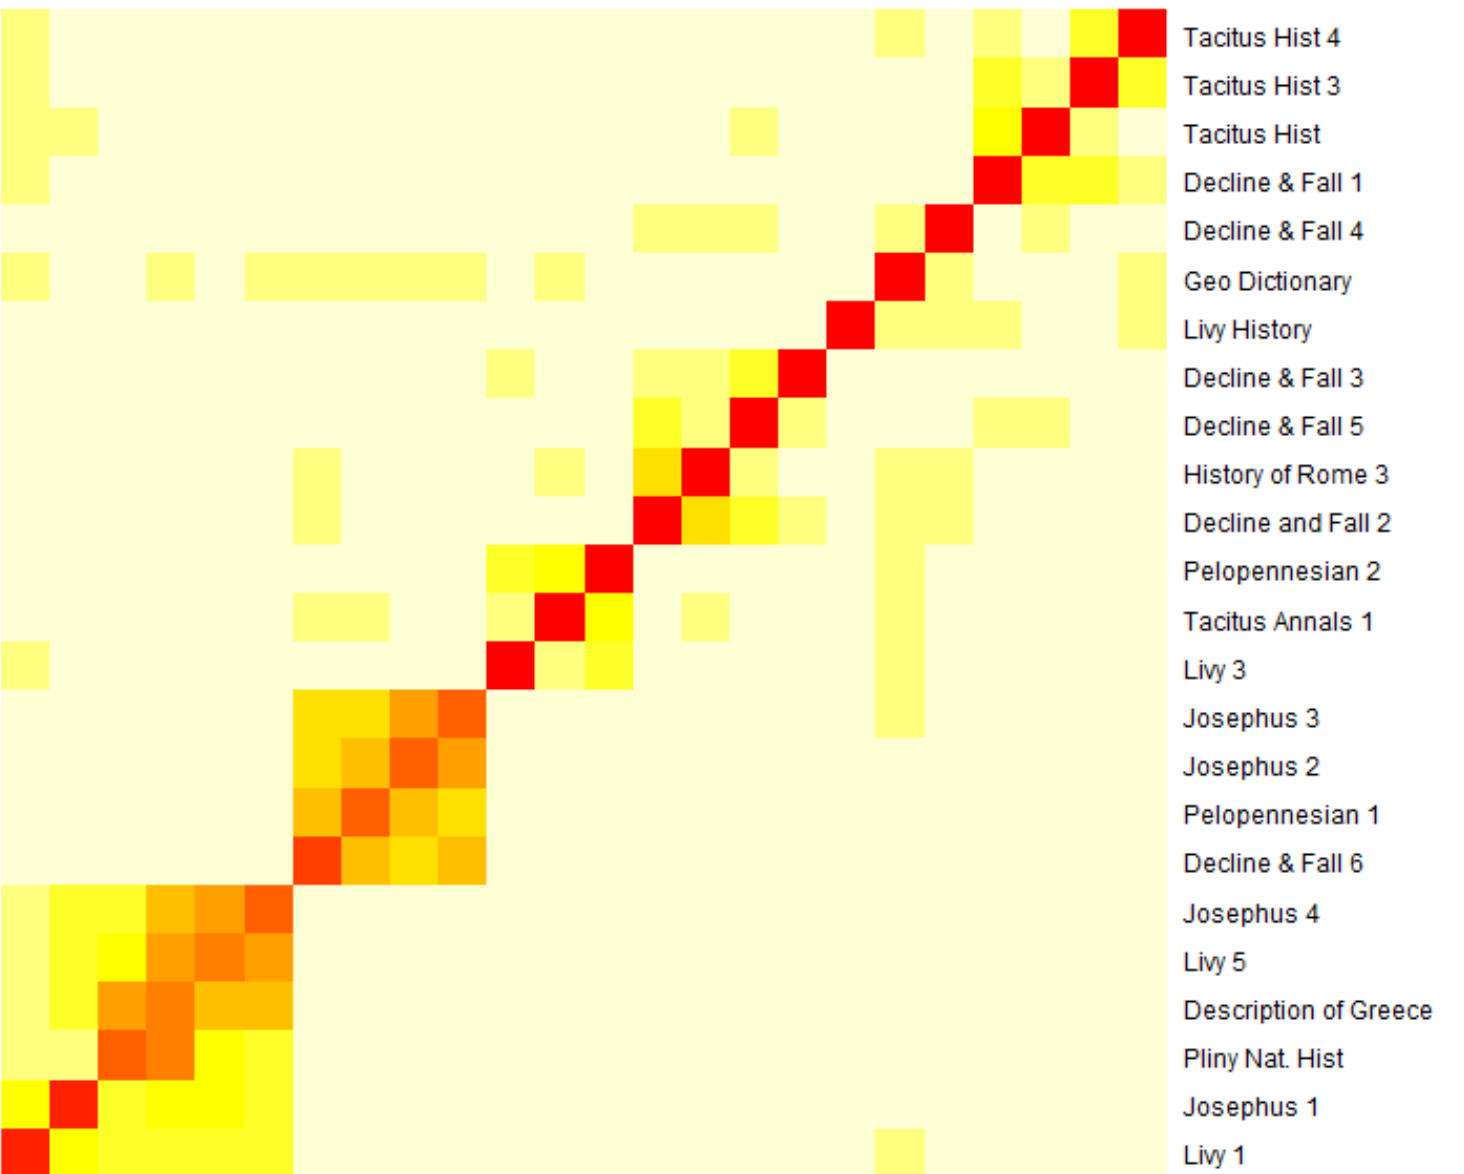
\includegraphics[width=\linewidth]{heatmap2.png}
	\caption{K-means clustering plotted on First two principal components. Using cluster package in R. Documents in clusters 1 and 3 are labelled\footnote{Other dimensional scaling techniques such as HDS also computed but with little additional information gained w.r.t. PCA}}
	\label{fig:kmeans}
\end{subfigure}%

\begin{subfigure}{.3\textwidth}
\centering
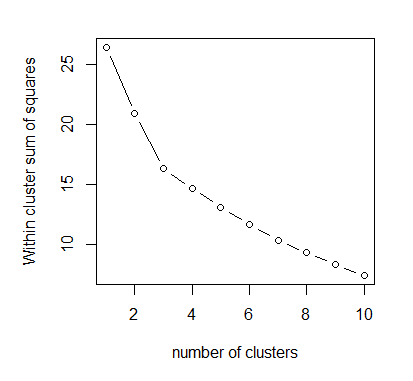
\includegraphics[width=\linewidth]{elbow.png}
\caption{Elbow plot varying number of clusters vs. within cluster spread}
\label{fig:elbow}
\end{subfigure}%

\begin{subfigure}{.3\textwidth}
	\centering
	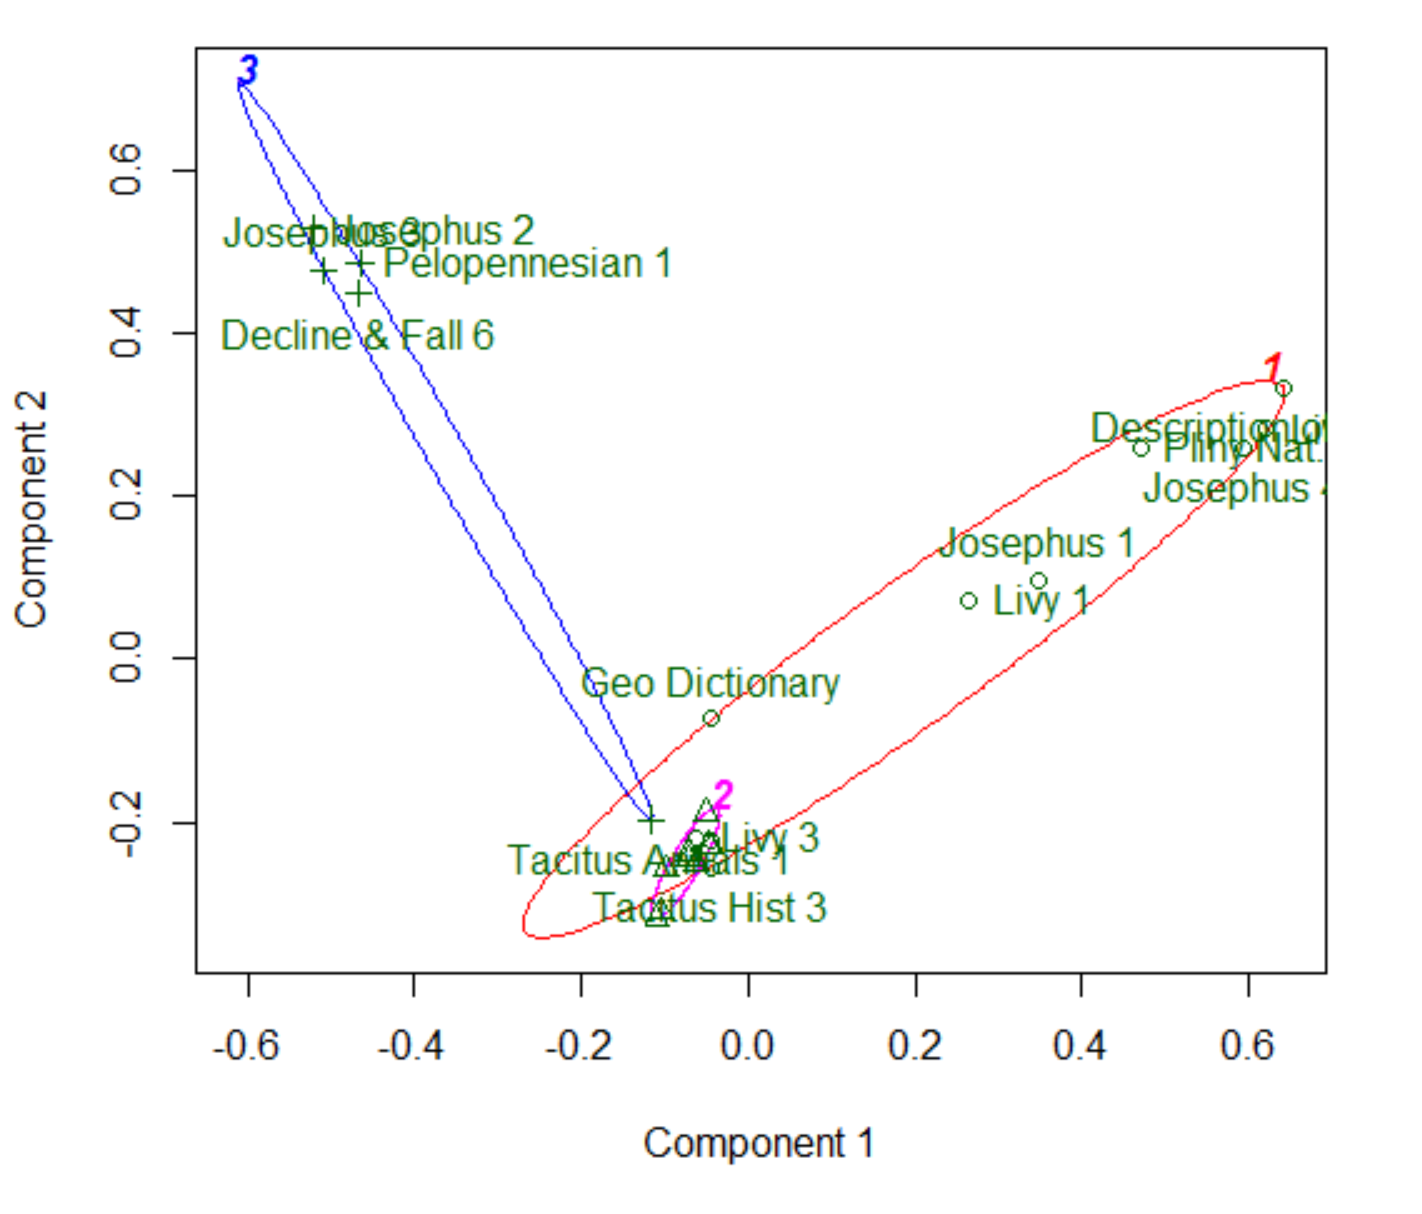
\includegraphics[width=\linewidth]{Kmeans.png}
	\caption{Heatmap of cosine dissimilarity matrix of each document.}}
	\label{fig:heatmap}
\end{subfigure}%

\begin{subfigure}{.3\textwidth}
	\centering
	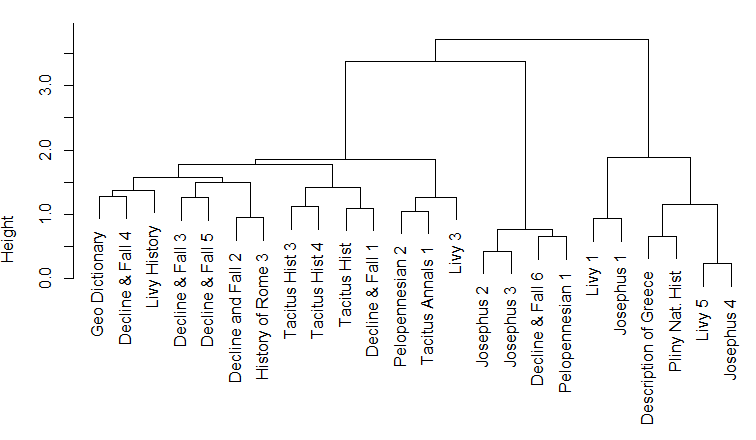
\includegraphics[width=\linewidth]{dendorgram.png}
	\caption{Dendrogram of agglomerative hierarchical  clustering using "Ward" method and cosine distance. Produced from cluster package in R.}
	\vskip -6pt
	\label{fig:heir}
\end{subfigure}
\end{figure}


\bibliographystyle{abbrv}
\bibliography{sigproc}  % sigproc.bib is the name of the 
\end{document}
